\section{Open Job Shop Problem}
\subsection{Introduction}
\begin{frame}
  \frametitle{Problem definition}

  \begin{itemize}
    \item $m$ \textbf{jobs} have to processed by $n$ \textbf{machines}
    \item A job $i$ stays on a machine $j$ for an \textbf{operation} with start time $t_{ij}$ and duration $d_{ij}$
    \item The order in which a job is passed from machine to machine can be chosen arbitrarily.
  \end{itemize}

  Goal: \textbf{minimize} the total \textbf{makespan}, i.e. the time at which the last machine finishes its last operation.

 	

\end{frame}

\begin{frame}
	\frametitle{Example}
	
	\begin{columns}[c]
		\column{.4\linewidth}

Valid schedule for a 3x3-problem (3 jobs, 3 machines)

\textbf{makespan:} 23, matches lower bound

		\column{.6\linewidth}
\begin{figure}
	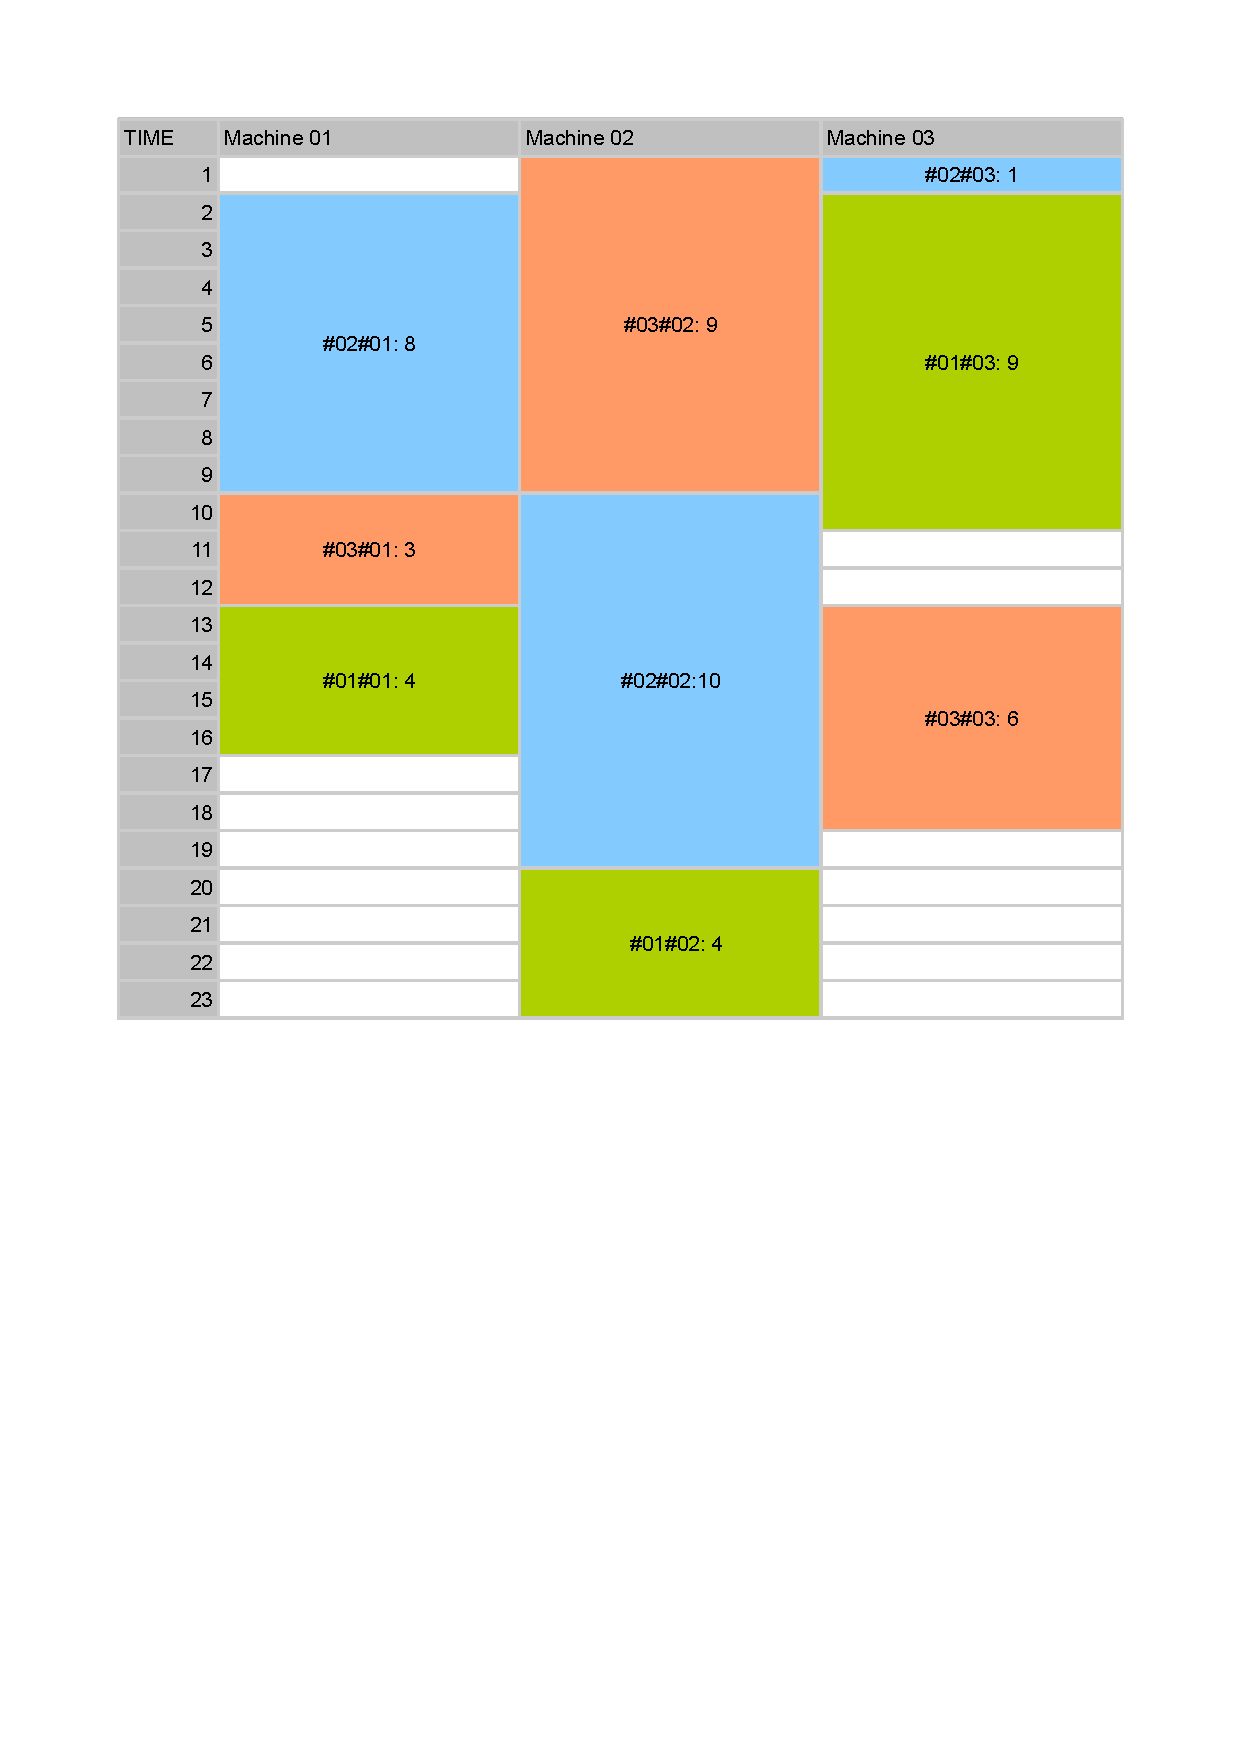
\includegraphics[width=\linewidth]{images/example-schedule.pdf}
	
\end{figure}
\end{columns}
	
\end{frame}

\subsection{Algorithms}
\begin{frame}
  \frametitle{Permutation Genetic Algorithm\cite{Khuri}}
	
	\begin{idea}
	
	
	\begin{itemize}
	
		\item Give each operation a unique $ID = 1,2,\dots, m \cdot n$

		\item 	Let the order of the IDs decide which operation is \textbf{scheduled} first.

		\item 	Use the \emph{genetic algorithm} to find the best \emph{permutation}.
	\end{itemize}
	
	\end{idea}
	
	\pause
	
	What does it mean to \emph{schedule} an operation?  

\end{frame}

\begin{frame}
  \frametitle{Scheduling step}
	
	
	\small
	\begin{columns}	
	\column{.5\textwidth}
Simple scheduling: Append operation to machine, after previous operations of the same job have finished.



\column{.5\linewidth}
	\begin{figure}
		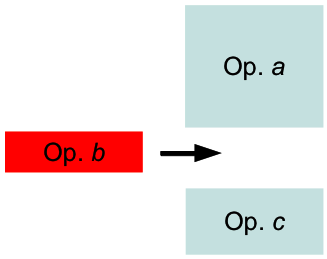
\includegraphics[width=.6\linewidth]{images/scheduling.png}

	\end{figure}
	
\end{columns}

\textbf{Better:} Use \textbf{gaps} (no other operation of the same job should be active)!

	A significant part of the optimization is ``hidden'' in this scheduling step!

\end{frame}

\begin{frame}
  \frametitle{Implementation details}
\begin{itemize}

	\item A chromosome consists of $m\cdot~n$ genes, each gene representing an operation.

	\item Start with random genes

	\item Genetic algorithm adapts genes freely as floats \textrightarrow the order of the genes decides the permutation, e.g.

	\item a chromosome $(64.4, 33.5, 64.5)$ represents the permutation $(2,1,3)$
\end{itemize}

\end{frame}

\begin{frame}
  \frametitle{Hybrid Genetic Algorithm}
\begin{itemize}

	\item 	Uses the same genetic algorithm with the same parameters, but

	\item  	permutes jobs instead of operations

	\item 	Keep a list of unfinished jobs, plus a list of unfinished operations for each of these jobs.

	\item 	All indices are modulo!
\end{itemize}
 
\end{frame}

\begin{frame}
  \frametitle{Why is it called hybrid?}
\begin{itemize}

	\item 	The lists of operations are sorted by duration \textrightarrow longest jobs are scheduled first!

	\item  	Performs well on big problems
\end{itemize}
 
\end{frame}

\begin{frame}
  \frametitle{Selfish Gene Algorithm}

\begin{itemize}

	\item Third approach from \cite{Khuri}%, does \textbf{not} use the evolib!

	\item [ Builds a virtual population ] instead of storing chromosomes, store probabilities of gene values.

	\item According to these probabilities, some genes are more likely to occur than others when an individual is picked.

	\item Two individuals are chosen and their fitness (makespan) compared. The genes of the winner are rewarded by increasing their probability.
	
	\item A \textbf{steady state} is reached when each gene acquires one value with a probability $\geq 95\%$
\end{itemize}

\end{frame}


\begin{frame}[fragile]
\vspace{-0.8cm}
{\scriptsize
\begin{verbatim}
SELFISH_GENE():
    
    population = [[1/m,1/n,...],[1/m,1/n,...], ...]
    best = choose individual from population
    
    FOR i = 1:max_iterations
        choose individual1, individual2 from population
        (winner, loser) = compare(individual1, individual2)
        reward(winner)
        punish(loser)
        IF fitness(winner) > fitness(best)
            best = winner
        END
        BREAK if steady_state(population)
    END
    
    RETURN best
\end{verbatim}}

\end{frame}

\begin{frame}
  \frametitle{Other approaches}
\end{frame}